\section{Wprowadzenie}

\subsection{Domain Specific Languages}


\begin{frame}
     \frametitle{Domain Specific Languages (DSL)}
     
     DSL to języki przystosowane do używania w konkretnym celu.
     \begin{itemize}
          \item
          łatwość użycia
          \item
          specyficzne konstrukcje
          \item 
          ograniczone możliwości
          \item
          kompilacja do języka niższego poziomu (np. SQL)
     \end{itemize}


\end{frame}

\section{Tabliczki sumeryjskie}
%Coś o sumerach


\begin{frame}
     \frametitle{Tabliczki sumeryjskie}

\begin{columns}
\column{0.5\textwidth}
\begin{itemize}
\item gliniane tabliczki pokryte pismem klinowym
\item pochodzą z terenów Bliskiego Wschodu
\item najstarsze znane pismo (powstało ok. 3500r. p.n.e.)
%\item wiele zachowało się dzięki pożarom, ważniejsze wypalano specjalnie
%\item odciskane rylcem o trójkątnym przekroju
\item pismo początkowo rysunkowe, później coraz prostsze
\item głównie teksty gospodarcze i administracyjne% (dość regularne i rzeczowe)

\end{itemize}
\column{0.5\textwidth}
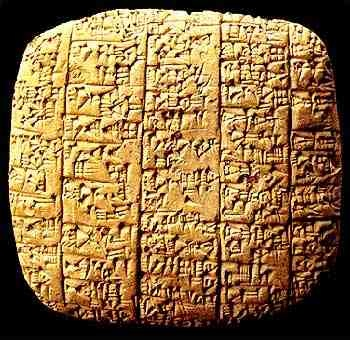
\includegraphics[width=55mm]{1/tablet.jpg}
\end{columns}
\end{frame}



\begin{frame}
\frametitle{Sumerologia}
    
\begin{columns}
 \column{0.5\textwidth}
Sumerologia to nauka badająca kulturę i historię starożytnych Sumerów, czerpiąca wiedzę m.in. z zachowanych tabliczek.
\begin{itemize}
\item zdigitalizowane i ręcznie skorygowane treści tabliczek są udostępnione przez system CDLI (obecnie prawie 225 000 tabliczek)
\item możliwość niewłaściwej interpretacji klinów
\item potrzebne intuicyjne narzędzie do wyszukiwania w bazie tabliczek na podstawie odczytów
\end{itemize} 

  \column{0.5\textwidth}
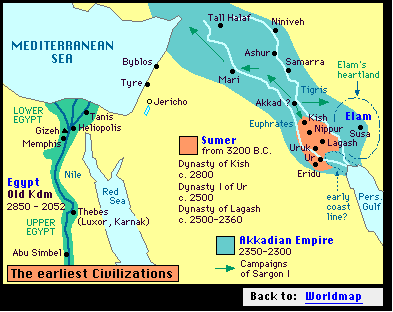
\includegraphics[width=55mm]{1/sum_map.png}
\end{columns}


\end{frame}


\section{Tablets Query Language}


\begin{frame}
     \frametitle{Tablets Query Language}
     \begin{itemize}
    \item Język pozwalający sumerologom łatwo tworzyć zapytania w bazie tabliczek.\\
   \item  Prosta składnia zapytań.\\
 \item    Zapytania zawierają informacje tylko o treści tabliczek i ich metadanych.\\
  \item   Możliwość stworzenia implementacji na dowolną bazę przechowującą tabliczki.\\ %ułatwiamy to dzięki podziałowi kodu na moduły

 \end{itemize}

\end{frame}
 
\begin{frame}

% dać składnię

     \frametitle{Przykładowe zapytania TQL}

\begin{block}{przykład 1}

provenience: Ur*\\
period: "Uruk III"\\
genre: Administrative\\
text: udu + (szid / sipa) $--$ adad-tilati\\

\end{block}
\end{frame}



\begin{frame}
\frametitle{Przykładowe zapytania TQL}
\begin{block}{przykład 2}
provenience: Gar*\\
period: UrIII\\
genre: Administrative\\
text: udu/masz2\\
~\\
provenience: Ur\\
period: UrIII\\
text: sig4\\
\end{block}
\end{frame}

\begin{frame}
 \frametitle{Przykładowe zapytania TQL}
\begin{block}{przykład 3}
define\\
  provenience: Garshana\\
  period: UrIII\\
  text: "udu ban"/mash2\\
as "zwierzaki w Garshana"\\
~\\
search\\
  text: adad-tilati\\
in "zwierzaki w Garshana"\\
\end{block}
\end{frame}
